\documentclass[tikz,border=5pt]{standalone}
\usepackage{amsmath}
\usetikzlibrary{arrows.meta,decorations.pathmorphing,calc}
\definecolor{cellc}{RGB}{236,226,201}
\definecolor{bmc}{RGB}{120,170,215}
\definecolor{intc}{RGB}{190,55,40}
\definecolor{boundc}{RGB}{25,115,55}
\definecolor{grayt}{RGB}{95,95,95}
\begin{document}
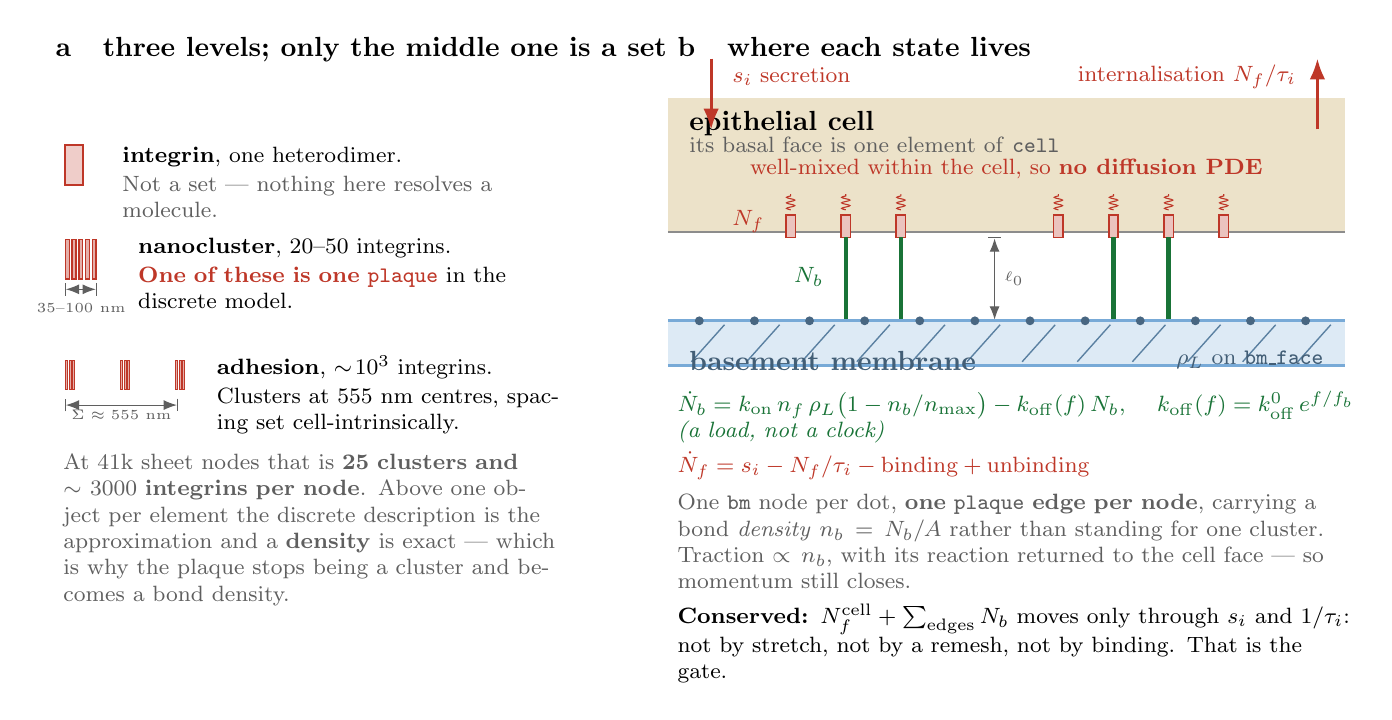
\begin{tikzpicture}[font=\small,>=Latex]

%================= a: the three levels =================
\node[anchor=north west,font=\bfseries] at (0,8.35) {a\quad three levels; only the middle one is a set};

\draw[fill=intc!25,draw=intc,line width=0.7pt] (0.25,6.35) rectangle ++(0.22,0.5);
\node[anchor=north west,align=left,text width=5.0cm,font=\footnotesize] at (0.85,6.95)
  {\textbf{integrin}, one heterodimer.\\[1pt]
   \textcolor{grayt}{Not a set --- nothing here resolves a molecule.}};

\foreach \i in {0,...,4}{\draw[fill=intc!40,draw=intc,line width=0.5pt]
   ($(0.25+0.085*\i,5.15)$) rectangle ++(0.05,0.5);}
\draw[grayt,|<->|] (0.24,5.02) -- (0.65,5.02);
\node[font=\tiny,text=grayt,anchor=north] at (0.45,4.96) {35--100 nm};
\node[anchor=north west,align=left,text width=4.9cm,font=\footnotesize] at (1.05,5.80)
  {\textbf{nanocluster}, 20--50 integrins.\\[1pt]
   \textcolor{intc}{\textbf{One of these is one \texttt{plaque}}} in the discrete model.};

\foreach \j in {0,1,2}{\foreach \i in {0,1,2}{\draw[fill=intc!40,draw=intc,line width=0.35pt]
   ($(0.25+0.70*\j+0.045*\i,3.75)$) rectangle ++(0.028,0.36);}}
\draw[grayt,|<->|] (0.24,3.55) -- (1.68,3.55) node[midway,below,font=\tiny,inner sep=1.5pt]
  {$\Sigma\approx555$ nm};
\node[anchor=north west,align=left,text width=4.6cm,font=\footnotesize] at (2.05,4.30)
  {\textbf{adhesion}, $\sim\!10^3$ integrins.\\[1pt]
   Clusters at 555 nm centres, spacing set cell-intrinsically.};

\node[anchor=north west,align=left,text width=6.4cm,font=\footnotesize,text=grayt] at (0.1,3.05)
  {At 41k sheet nodes that is \textbf{25 clusters and $\sim\!3000$ integrins per node}.
   Above one object per element the discrete description is the approximation and a
   \textbf{density} is exact --- which is why the plaque stops being a cluster and becomes a
   bond density.};

%================= b: where each state lives =================
\begin{scope}[xshift=7.9cm]
\node[anchor=north west,font=\bfseries] at (0,8.35) {b\quad where each state lives};

% --- cell block
\fill[cellc] (0,5.75) rectangle (8.6,7.45);
\draw[black!45,line width=0.9pt] (0,5.75) -- (8.6,5.75);
\node[anchor=north west,font=\bfseries] at (0.15,7.40) {epithelial cell};
\node[anchor=north west,font=\footnotesize,text=grayt] at (0.15,7.08)
  {its basal face is one element of \texttt{cell}};

% free integrins
\foreach \x in {1.5,2.2,2.9,4.9,5.6,6.3,7.0}{
  \draw[fill=intc!30,draw=intc,line width=0.6pt] (\x,5.68) rectangle ++(0.12,0.28);
  \draw[intc,decorate,decoration={coil,aspect=0,segment length=2pt,amplitude=1.5pt}]
    ($(\x+0.06,6.03)$) -- ++(0,0.20);}
\node[anchor=east,text=intc,font=\footnotesize] at (1.35,5.88) {$N_f$};

\draw[intc,<->,line width=0.7pt] (1.56,6.55) -- (7.06,6.55);
\node[font=\footnotesize,text=intc,fill=cellc,inner sep=1.5pt] at (4.3,6.55)
  {well-mixed within the cell, so \textbf{no diffusion PDE}};

\draw[->,intc,line width=1.0pt] (0.55,7.95) -- (0.55,7.05);
\node[anchor=west,font=\footnotesize,text=intc] at (0.70,7.72) {$s_i$ secretion};
\draw[->,intc,line width=1.0pt] (8.25,7.05) -- (8.25,7.95);
\node[anchor=east,font=\footnotesize,text=intc] at (8.10,7.72) {internalisation $N_f/\tau_i$};

% --- bonds
\foreach \x in {2.2,2.9,5.6,6.3}{
  \draw[boundc,line width=1.6pt] (\x+0.06,5.68) -- (\x+0.06,4.62);
  \draw[->,boundc,line width=0.9pt] (\x+0.06,4.62) -- ++(0,-0.30);}
\node[anchor=east,text=boundc,font=\footnotesize] at (2.10,5.18) {$N_b$};
\draw[grayt,|<->|] (4.15,4.62) -- (4.15,5.68);
\node[font=\tiny,text=grayt,anchor=west,inner sep=2pt] at (4.20,5.15) {$\ell_0$};

% --- sheet
\fill[bmc!25] (0,4.05) rectangle (8.6,4.62);
\draw[bmc,line width=1.2pt] (0,4.62) -- (8.6,4.62);
\draw[bmc,line width=1.2pt] (0,4.05) -- (8.6,4.05);
\foreach \x in {0.3,1.0,1.7,2.4,3.1,3.8,4.5,5.2,5.9,6.6,7.3,8.0}{
  \draw[bmc!75!black,line width=0.5pt] (\x,4.10) -- ++(0.42,0.47);}
\node[anchor=north west,font=\bfseries,text=bmc!55!black] at (0.15,4.36) {basement membrane};
\node[anchor=north east,font=\footnotesize,text=bmc!55!black] at (8.45,4.36)
  {$\rho_L$ on \texttt{bm\_face}};
\foreach \x in {0.4,1.1,1.8,2.5,3.2,3.9,4.6,5.3,6.0,6.7,7.4,8.1}{
  \fill[bmc!60!black] (\x,4.62) circle (1.6pt);}

% --- the text, clear of the drawing
\node[anchor=north west,align=left,text width=8.6cm,font=\footnotesize] at (0,3.85)
  {\textcolor{boundc}{$\dot N_b=k_{\rm on}\,n_f\,\rho_L\bigl(1-n_b/n_{\max}\bigr)-k_{\rm off}(f)\,N_b$,
   \quad $k_{\rm off}(f)=k^0_{\rm off}\,e^{f/f_b}$ \ \textit{(a load, not a clock)}}\\[3pt]
   \textcolor{intc}{$\dot N_f=s_i-N_f/\tau_i-\text{binding}+\text{unbinding}$}\\[4pt]
   \textcolor{grayt}{One \texttt{bm} node per dot, \textbf{one \texttt{plaque} edge per node},
   carrying a bond \emph{density} $n_b=N_b/A$ rather than standing for one cluster. Traction
   $\propto n_b$, with its reaction returned to the cell face --- so momentum still closes.}\\[3pt]
   \textbf{Conserved:} $N_f^{\rm cell}+\sum_{\rm edges}N_b$ moves only through $s_i$ and $1/\tau_i$:
   not by stretch, not by a remesh, not by binding. That is the gate.};
\end{scope}
\end{tikzpicture}
\end{document}
